%% The following is a directive for TeXShop to indicate the main file
%%!TEX root = diss.tex

\chapter{Problem Space of 3D Reconstruction}
\label{ch:3DRecon_Taxo}
Existing taxonomies of 3D reconstruction techniques generally classify algorithms based on algorithmic details: the survey on Multi-view Stereo algorithms uses taxonomies that differentiate the key properties of each algorithm~\cite{seitz2006comparison}. Reviews on Structured Light techniques typically classify techniques based on the type of projection pattern used~\cite{geng2011structured, salvi2004pattern}. Photometric Stereo algorithms are classified by the assumptions or generalizations made, such as, unknown/known reflectance, unknown/known light conditions (uncalibrated/calibrated), and so on~\cite{shi2016benchmark}.
However these taxonomies have the following limitations: 1) they are algorithm centric, classifying algorithms based on \textit{how} an algorithm solves the problem, giving little to none insight to the conditions that allow a specific algorithm to work well, thus requires vision knowledge to fully take advantage of these algorithms; 2). they provide means to categorize within-category algorithms, but are unsuitable to compare the performance of between-category algorithms. It is well known that such algorithms target limited categories of objects, and are highly likely to fail when targeting a diverse set of object categories. It is crucial to understand the conditions a specific algorithm performs well when designing an application for reconstruction. Under the previous framework of taxonomy, this knowledge is largely empirical, with each algorithm mapped roughly to a sub-volume in the problem space that is poorly defined. To overcome these limitations, we take a more \textit{object-centered approach} instead of an \textit{algorithm-centered approach}.

The taxonomy proposed in this chapter defines 3D reconstruction techniques from an object-centered viewpoint, \ie categorizes algorithms based on the problem conditions that it can reliably work under. This taxonomy transforms the 3D reconstruction problem from one requiring knowledge and expertise of specific algorithms in terms of \textit{how} to use them, to one requiring knowledge of working conditions of each algorithm.

\section{Problem space}
The proposed object-centered taxonomy categorizes algorithms based on the type of objects/problem conditions that they can reliably work under. We first give an overview of object classes, which serves as the bases to the taxonomy, then proceeds to investigate the working conditions of each class of algorithms based on relevant literature reports.

In Figure~\ref{fig:obj_class}, we show a taxonomy of object classes based on material and shape properties. However, by no means are these presented object classes complete. There are many other properties not included that are commonely seen in the real world. For instance, effects such as occlusion, discontinuity, and emission, among others, are not considered. Further, we assume \textbf{local interaction model}, \ie global light transport such as transmission, refraction, cast shadow, inter-reflection are not considered. The rationale behind our choice is that most techniques that have been developed over the past few decades mainly tackle object with an opaque, diffuse or mixed surface. For specular, refractive, and translucent or transparent objects, only very specialized algorithms are applicable for reconstruction~\cite{ihrke2010transparent}. We propose the following labels to differentiate object classes. The order of properties for the class label is as follows: translucency, texture, lightness, reflectance model, surface roughness, and concavity. To approach this problem in a feasible manner, four classes of objects are being investigated in depth. They are selected based on the availability of reliable techniques and the diversity of corresponding real-world objects.
\begin{figure}[!htbp]
\centering
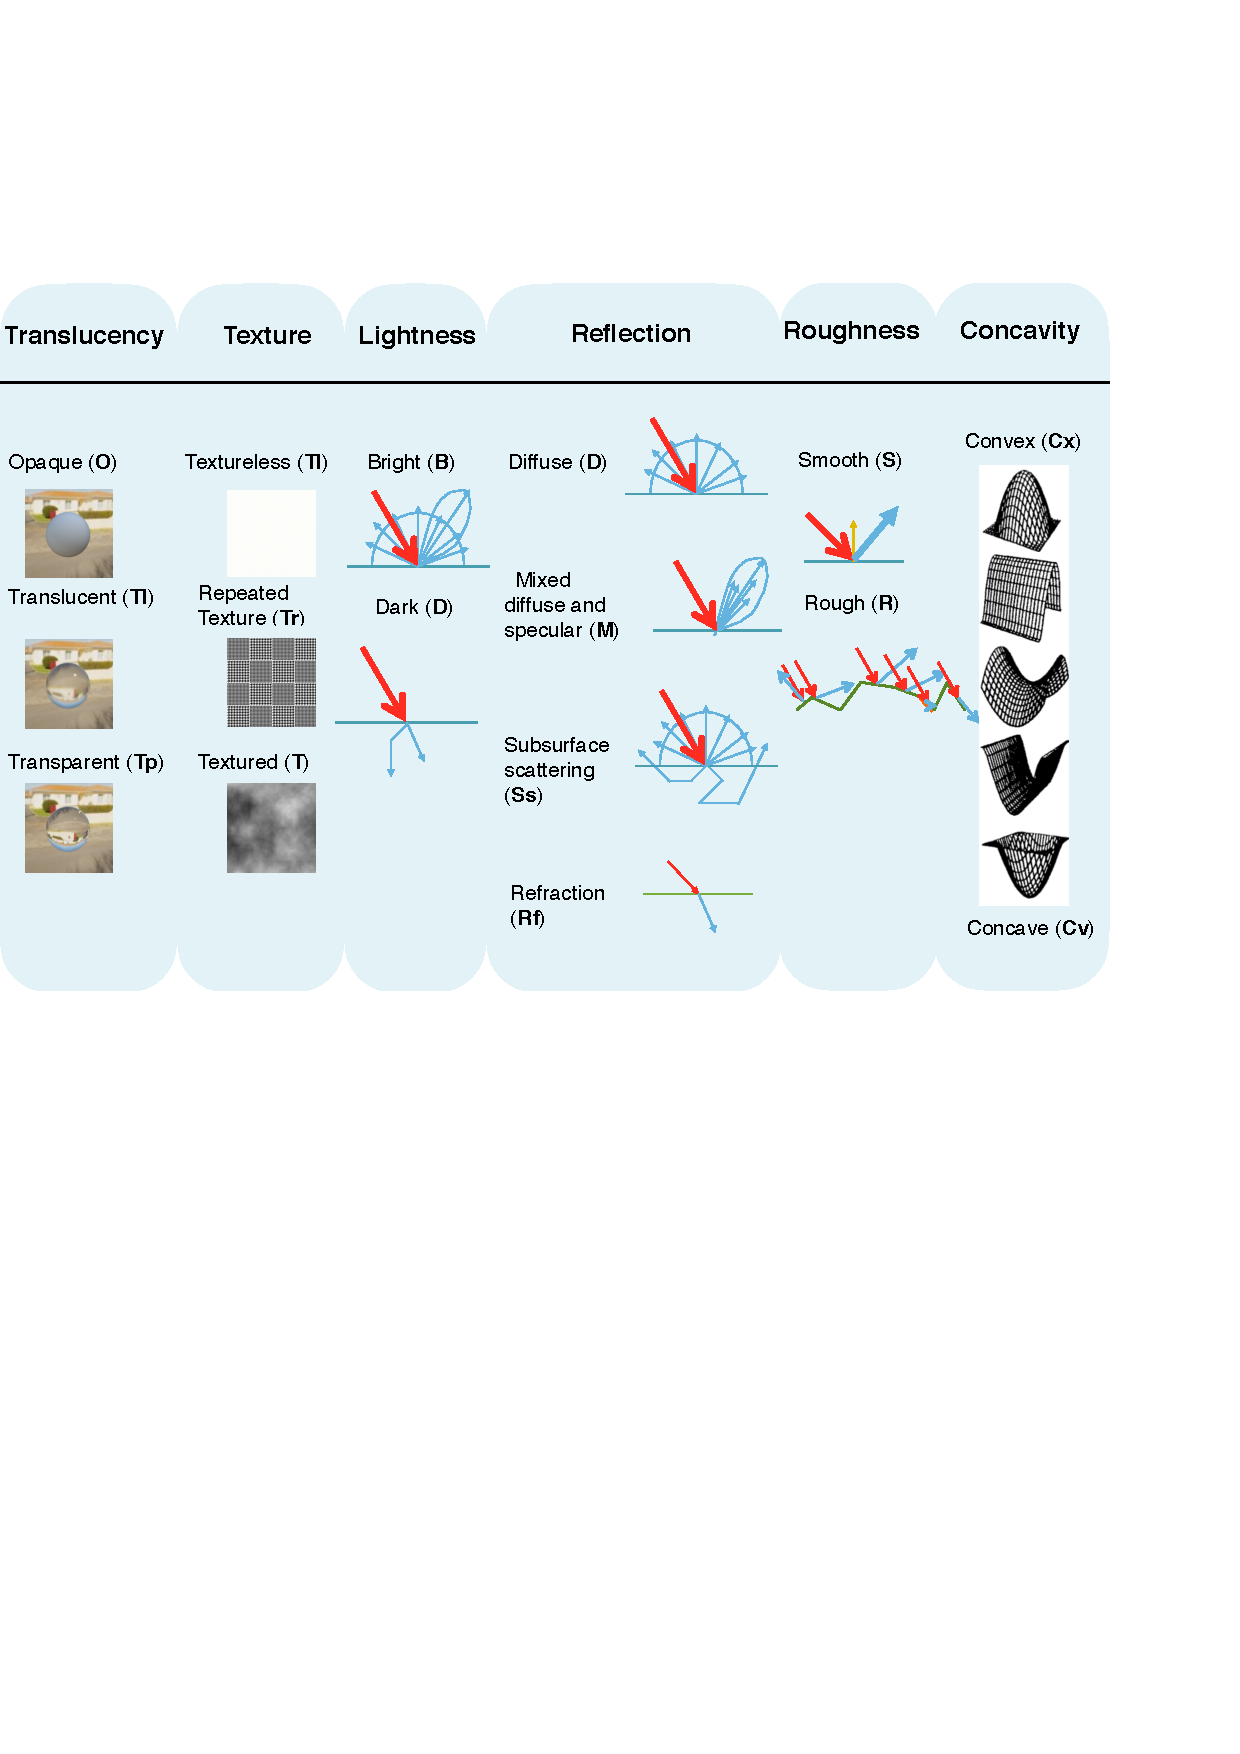
\includegraphics[width=\textwidth]{taxo/obj_class}\\
\caption{A list of properties for object classes.}
\label{fig:obj_class}
\end{figure}

\subsubsection{Labels of Properties}
\begin{itemize}
\item \textbf{Translucency}: \textbf{O}: opaque, \textbf{Tl}: translucent, \textbf{Tp}: transparent.
\item \textbf{Texture}: \textbf{T}: textured, \textbf{Tr}: repeated textured, \textbf{Tl}: textureless.
\item \textbf{Lightness}: \textbf{B}: bright, \textbf{D}: dark.
\item \textbf{Reflection}: \textbf{D}: diffuse model, \textbf{S}: specular model, \textbf{M}: mixture of diffuse and specular, \textbf{Ss}: subsurface scattering, \textbf{Rf}: refraction
\item \textbf{Roughness}: \textbf{S}: smooth, \textbf{R}: rough
\item \textbf{Concavity}: \textbf{Cx}: convex, \textbf{Cv}: concave
\end{itemize}

\section{Scope}
To limit the scope of this work, we make the following assumptions:

\subsection{Simplified reflectance model}
Since the majority of reconstruciton techniques rely on observing light reflected off a surface, surfaces exhibit significant effect of global light tranport present a huge challenge to the reconstruction problem. Surface exhibits global light transport, including \textit{specular}, \textit{transmission}, \textit{sub-surface scattering}, \textit{inter-reflection}, \textit{self-shadow}, and etc would break the assumptions made by most generic 3D reconstruction algorithms. Thus the global light transport are ignored, and the reflection properties of consideration are \textit{albedo}, \ie the ratio of reflected light w.r.t the received light, and \textit{specularity}, \ie the amount of specular reflection. A more comprehensive model should be constructed based on our work to incorporate more complex phenomena to be more comprehensive.

\subsection{Simplified geometric model}
It's a challenging task to model geometry using mathematical descriptions. For geometric primitives such as cube, sphere, or cone, etc, it's possible to describe the shape using concise descriptions. However, the task becomes prohibitive when it comes to shapes with varied characteristics. Furthermore it becomes more ambiguous when natural language is employed. Thus we only consider the microscopic roughness of the surface, which has a direct relation with the reflection. Other prominent geometric properties such as \textit{concavity}, which affects self-shadow, inter-reflection, \textit{depth-discontinuity}, which affects the depth estimation, are ignored.

\subsection{Simplified object class}
Only a subset of visual/geometric properties are considered, which include texture, lightness, specular, and roughness. Since we use a simplified reflectance and geometric model, phenomena such as translucency, subsurface scattering, refraction, occlusion, concavity can not be described properly. Thus object exhibiting those properties are not considered in the evaluation.

\section{Summary}
Our taxonomy categorizes algorithms based on the problem conditions that they can reliably work under. The problem conditions consist of various visual and geometric properties, as shown in Figure~\ref{fig:obj_class}. These properties can be conceptualized as dimensions of the 3D reconstruction problem space. This taxonomy provides an abstraction which allows us to think of algorithms as volumes within an $n-$dimensional problem space. Existing algorithms can be introduced into this framework based on the performance within the problem space. The aforementioned analysis provide an initial mapping of the space that is summarized below in Figure~\ref{fig:prob_cond}.
\begin{figure*}[!htbp]
\centering
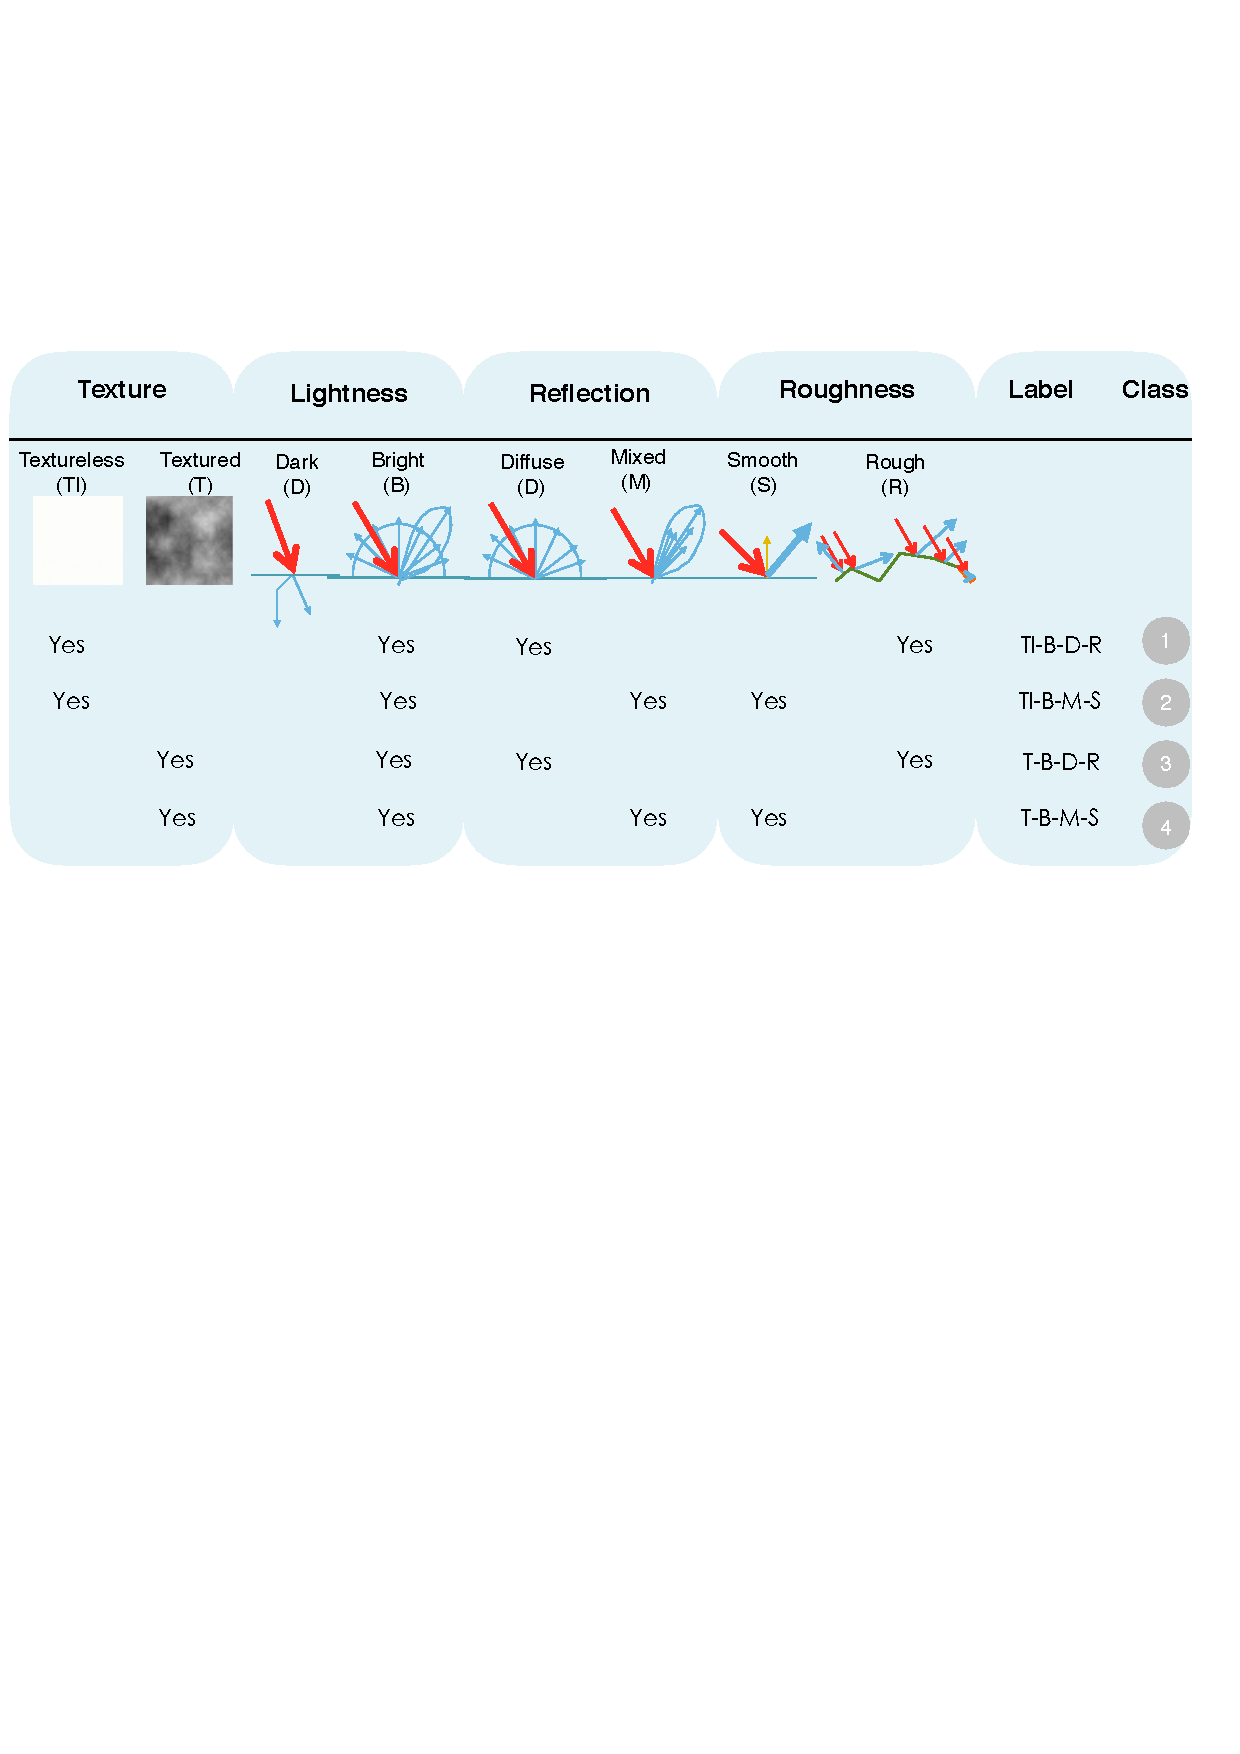
\includegraphics[width=0.8\textwidth]{taxo/prob_cond}
\caption{Four classes of problem conditions of interest with the proposed label.}
\label{fig:prob_cond}
\end{figure*}